\chapter{Objetivos}
\label{cap:Objetivo}
A continuación se expone el objetivo de este trabajo así como una serie de objetivos parciales que se pretenden alcanzar durante el desarrollo y que toman parte en el objetivo principal.
\section{Objetivo Principal}
El objetivo principal de este \gls{TFG} es la construcción de un sistema inteligente para la simulación de la \textbf{distribución óptima} de energía entre \textbf{elementos generadores} y \textbf{elementos consumidores} en el hogar.\\
Las fuentes de suministro de energía (elementos generadores) son:
\begin{itemize}
	\item Módulos fotovoltaicos
	\item Red eléctrica
	\item Baterías de almacenaje
\end{itemize}
Como fuentes de consumo (elementos consumidores) existen:
\begin{itemize}
	\item Consumo energético del hogar
	\item Consumo propio del sistema que se propone
	\item Carga de baterías de almacenaje
	\item Venta al mercado eléctrico como particular
\end{itemize}
En la Figura~\ref{fig:schema} se muestra un esquema del sistema para facilitar la compresión de su funcionalidad. El sistema debe ser capaz de ajustar automáticamente en cada momento la cantidad de energía obtenida de los mencionados anteriormente con el objetivo de minimizar el gasto económico dedicado en el hogar.

\begin{figure}[!h]
	\centering
	\includegraphics[width=7cm]{figs/Esquema.png}
	\caption{Esquema del sistema}
        \label{fig:schema}
\end{figure}

\section{Objetivos Parciales}
A lo largo del trabajo habrá que satisfacer una serie de subobjetivos necesarios para lograr el objetivo principal tales como:
\begin{enumerate}
	\item \textbf{Identificación y adquisición de los datos y variables que definen el sistema:}
	Estudio de las entradas del sistema y el grado de importancia que tiene cada una en cada situación. La información meteorológica será obtenida utilizando una \gls{API} oficial de \gls{AEMET}~\cite{Aemet}, y los datos del mercado eléctrico serán obtenidos utilizando la \gls{API} oficial e-sios de \gls{REE} S.A.~\cite{Ree}

	\item \textbf{Establecer las relaciones y restricciones propias del modelo:}
	Las variables obtenidas en el objetivo anterior estarán sujetas a unas restricciones que nos permitirán conocer las combinaciones posibles de valores, teniendo en cuenta que toda la energía generada debe ser consumida de alguna forma, ya sea por medio de venta a la red, o cargada en baterías de almacenaje en caso de superar la energía demandada por el consumo que se realiza.

	\item \textbf{Añadir una inteligencia artificial para la generación optimizada de energía y dar lugar a una planificación:}
	Una vez obtenidos los datos y variables del problema y conociendo el grado de implicación de los mismos, se creará un modelo del sistema que dará una planificación temporal de 24 horas. Esto se podrá llevar a cabo incorporando inteligencia artificial.

      \item \textbf{Hacer usable el sistema para realizar simulaciones a demanda:}
        Una vez se disponga de la funcionalidad de realizar simulaciones, se creará una aplicación web que permitirá interactuar a usuarios con el sistema, pudiendo realizar simulaciones de un día concreto y comparar los resultados obtenidos con lo ocurrido realmente a través de la compañía eléctrica.

      \item \textbf{Integración del sistema en la nube:}
        Cuando se cuente con una aplicación funcional, deberá integrarse en la nube para no tener dependencia de una máquina concreta haciendo honor a la tendencía cada vez más extendida del \textit{cloud computing}.

\end{enumerate}
